The second modelinvestigated was proposed by Chen \textit{et al}. \cite{chen2021shape}, 
building on the work of Spagnolie \textit{et al}. 
\cite{spagnolie2015geometric}. This advances  on the previous model by incorporating hydrodynamic interactions
with the channel walls into the SDEs for the cell.

Spagnolie \textit{et al.} approximate the velocity field around an elliptic swimmer by first treating the system as a 
\textit{stresslet} - a force dipole - and then by Faxén's Law obtaining the corresponding velocity field for a 
swimmer with elliptic shape. Figure shows two illustrative charts of a microswimmer treated as a stresslet, and the 
velocity field around this elliptic stresslet near the boundary. 

\begin{figure}[htbp]
    \centering
    \begin{subfigure}[b]{0.45\textwidth}
        \centering
        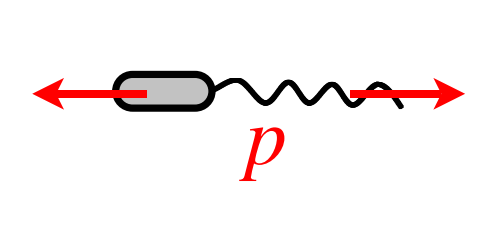
\includegraphics[width=\textwidth]{graphics/pusher_pic.png}
        \caption{Stationary}
        \label{fig:pusher_chart}
    \end{subfigure}
    \hfill
    \begin{subfigure}[b]{0.45\textwidth}
        \centering
        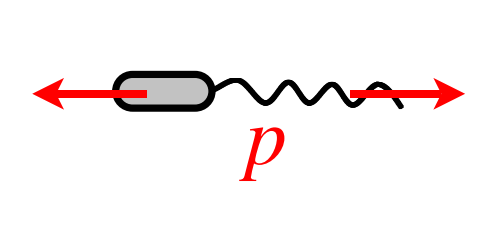
\includegraphics[width=\textwidth]{graphics/pusher_pic.png}
        \caption{Marginal}
        \label{fig:fluid_field_pusher}
    \end{subfigure}
    \caption{Comparison of stationary distribution and its marginal along $y$.}
    \label{fig:model_2_intro}
\end{figure}

% It is worth noting that in the literature microswimmers are categorised as either 
% \textit{pushers} 